\documentclass{report}
\usepackage[utf8]{inputenc}
\usepackage[english]{babel}
\usepackage{csquotes}
 	
\usepackage{graphicx}
\usepackage{booktabs} % for nice tables
\usepackage{multirow}

\usepackage{amsmath}

\usepackage{qtree}
\usepackage{tikz}
\usepackage{tikz-qtree}

\usepackage[hidelinks]{hyperref}
\usepackage[a4paper, margin=25mm]{geometry}
\usepackage{rotating}
\usepackage{pdflscape}
\usepackage{afterpage}
\usepackage{graphicx}

\usepackage[toc,page]{appendix}


\begin{document}

\begin{titlepage}
    \begin{center}

        \vspace*{1cm}
        \Huge
        \textbf{Reconstructing families - Bachelor Thesis}

        \vspace*{5cm}

        \LARGE
        \textbf{C.W. Joosse}\\
        4158407\\
        \today
        \vfill
        \Large
        UTRECHT UNIVERSITY\\
        Artificial Intelligence\\
        \vspace*{0.5cm}
        Supervisor: dr. ir. Gerrit Bloothooft\\
        Second supervisor: dr. Marijn Schraagen\\

        \vspace*{1cm}
        \large
        Bachelor thesis - 15 ECTS\\
    \end{center}
\end{titlepage}

\abstract{Edit distance is often used in record linkage for real persons to express the similarity of two names. In historical data names often have high spelling variance. This study investigates a method to deal with high name spelling variance by using overlinking and filtering in order to generate matches on a dataset of historical civil registrations. The method tries to build sets of registrations of persons that belong to the same family by applying real world knowledge to the generated matches. When using the four names of the parents mentioned on the registrations and an edit distance of 4 and 5, 80\% to 85\% of the generated matches are consistent with real world knowledge.}

\tableofcontents

\chapter{Introduction}
In the last decades, technological progress has given rise to new developments in the field of data science. Computers are used extensively in our daily lives, and the amount of information available on the internet is ever increasing. This data can be used by universities, companies and governments to find patterns in human behaviour. Due to increased computing power of processors, increased storage capacities and programming techniques that are focussed around distributed computing, organizations more capable then ever to analyse this data. \\
This data is often stored in data warehouses, where each unit of data is stored in a structured way. Although data architecture practices describe some form of data normalization, most data warehouses are not necessarily compatible with each other and therefore most data concerning the same entity is often stored in a slightly different way across different data warehouses. More than ever, analysis of data often requires that different data sources should be joined in order to create more enriched data sets and to discover new links between data. \\

In order to link data sources with each other these data sources should be able to identify which entity in one data source can be coupled to the same entity in the other data source. However, data is not saved according to a universal standard and because of this, each source could save the same information in a different format, making it harder to link this data. \\ Humans usually are capable of deciding whether two data records refer to the same entity, because they have knowledge about the context and have acquired knowledge about the world.
However, matching data using humans will often require too much time and is therefore expensive, and it is often left to computers to do this task. The problem of combining records from the same data source, or from different data sources and finding data that are about the same entity is called \textit{Record Linkage}. \\

When the keys in two data sources do not correspond with each other, alternatives must be used to identify entities, and very often, the task of linking records becomes non-trivial. In the case of entity resolution of persons, this often boils down to personal information such as date of birth, addresses and names. These data are often prone to errors, such as typographical errors or variations, outdated information or the fact that some databases are not allowed to store certain information due to legislation. \\

Given these problems, record linkage techniques often use knowledge from several research fields. For example: in order to cope with typographical variations and errors, method developed by linguistics can be used, whereas the computer sciences can provide techniques to deal with large amounts of data in an efficient way. When a link has been established, statistical methods can be used to provide a certain degree of certainty about the correctness of a link. This places the field of record linkage in the domain of artificial intelligence, which aims to combine these reseach fields to provide a comprehensive method to model intelligent behaviour which, for instance, can be applied in computer software.

This report will focus on applying record linkage techniques on historical data. Historical data often brings an extra set of problems: most of the modern data modeling techniques where not applied, and often data is missing or stored in an incoherent method. 

\section{Overview of research on record linkage}
The term \textit{record linkage} was introduced by Dunn \cite{dunn1946record}, who wanted to assemble a `book of life' for each person which would describe the person's interaction with health and social security systems, and which would also contain the birth-, death- and marriage-certificates of that person. In 1969 Ivan Fellegi and Alan Sunter \cite{fellegi1969theory} proved that, when the attributes that are used in the comparison are independent of each other, a optimal probabilistic decision rule can be found. This work has been the cornerstone of much of the data matching systems that are used today. Their model classifies two records \textit{a} and \textit{b} as either a match, non-match or possible match, based on a decision function that computes the probabilities for each class. They suggested that the set of possible matches should be held under clerical review, in order to classify the records in that class as either a match or as non-match. Since this involves human decision making, which is not fail-safe.\\ 

\cite{newcombe1962record} introduces the concept of \textit{blocking} to the field of record linkage, by showing how to reduce the number of pairs to link to consider only those pairs that agree on some characteristics. \cite{levenshtein1966binary}, \cite{jaro1989advances} and \cite{winkler1990string} introduced methods to calculate string similarity. These techniques are widely used in automated matching algorithms.\\

In more recent years a lot of research has focused on using machine-learning algorithms for record linkage. \cite{sarawagi2002alias} described a method to use an active learning algorithm that minimizes human input when constructing similarity functions. \cite{winkler2002methods} used the Expectation-maximization algorithm and a bayesian network for record linkage in a unsupervised learning setting. \\

Examples of research that specifies on string matching for person names can be found in \cite{zobel1996phonetic}, who showed that more efficient matching on person names can be achieved when using phonetic forms of names. They introduced improvements on the standard Soundex (\cite{russell1918soundex}) to rewrite person names. \cite{bloothooft2014learning} also introduced rules to improve person name matching, based on the edit distance of the names when the names have been rewriten in semi-phonetic form. These rules to rewrite names into semi-phonetic form have been introduces by \cite{bloothooft1995rules}\\

In \cite{Aspects001} a method was proposed in order to link registration certificates of the life events from the \textit{Genlias} project. Since the persons in this data set are not provided with an unique id, matching of records is done by matching the names that appear on the certificates. This approach groups the certificates where the names of the persons that are similar to each other in an efficient way. Matches are found by calculating the edit distance between the names that occur on both certificates.\\

\section{The Genlias project}
Throughout history, governments held censi and civil status to identify civilians and keep records about them, in order to register taxations and the people that are allowed to vote, for example. So did the government of The Netherlands in the $18^{th}$ and $19^{th}$ century. During that time, The Netherlands was occupied by the Frence empire of Napolean Bonaparte. The French introduced the `Burgerlijke stand'; the civil status in the Netherlands, which was responsible for recording births, marriages and deaths of the inhabitants of the Netherlands. 

Census are often a very valuable source of information, as they show the state of the population at a given point in time. Civil registrations however provide more information about the development of the population, such as migration patterns and health statistics.

The \textit{Genlias} project is a project that has started in the last decade of the $20^{th}$ century with the aim to collect all the certificates that where produced into a single database. This database is available via \url{http://www.wiewaswie.nl}. \newline

The dataset gives us great insight into the population of the Netherlands in the $19^{th}$ century. However, unlike more modern registration practices, the original records form the civil status are not provided with unique identification numbers, which makes it harder to do research. Another complicating factor is that it was not uncommon for officials to write different names for the same person on different registrations. When people married, for example, the persons involved would be registered with the official names. However, when a person passed away, it could happen that the neighbors of that person had to report this event to the civil registration. These neighbors didn't always know the full official birth names of the person deceased.\\ 

Using record linkage to resolve the life events of the persons recorded in the Genlias dataset could give researchers invaluable information about the population of the Netherlands in the $19^{th}$ century. Examples of interest are infant mortality rates for health research or migration patterns and (social) mobility for economical and social research.

\section{An overview of the method}
The subject of this thesis is to find a method for matching names that have a high chance of spelling variations in the absence of a golden standard. In particular, by using the method proposed by \cite{Aspects001} and increasing the allowed edit distance, applying a set of rules on names of the generated matches and by applying checks that are generated from domain knowledge, this thesis will test if it is possible to be resistant to spelling variance in names and still generate reliable matches by checking if the resulting matches do correspond to knowledge about the real world. \\

The linkage of registrations is done in three phases. First, for each marriage certificate a set of potential matching certificates (targets) is build by matching the names of the bride and groom on each target certificate to the names of the parents on the candidate certificates, using the method that was described by \cite{Aspects001}. The candidate certificates consists of all the known certificates: all the birth, marriage and death certificates in the Genlias project for the province of Zeeland. In the case of a marriage registration, both the parent couples for the groom and bride are checked against a target certificate. 
The (levenshtein) edit distance can be used to regulate how strict the names should match each other.\\
Since the candidate registrations are always checked against the same target registrations of parents, the resulting links can be seen as a set of events in the lifes of the children of the parents that are mentioned on the target registration to which they are matched. The linking procedure will result in a mapping from a target registration to a set of candidate registrations. This set of registrations will be refered to as a `family'.\\

In the second phase, the four individual names on the links generated in the first phase are compared to each other. Links where the names differ too much are removed from the set. The third phase is to check the resulting matches against a set of rules, which are based on domain knowledge, in order to determine how well the registrations in the set of families can correspond to actual life events. For instance, it is very unlikely (if not impossible) for a child to be born fifty years after the father and mother have been married. The set of rules will filter out these links that are not consistent with a normal flow of life events.\\

The quality of the matching results will be evaluated based on the acceptance rate in the third phase. Since there is no golden standard available of true matches on the Genlias dataset, it is not possible to compute the regular performance standards, such as precision, recall or reduction ratio, as it is not clear what the matches and non-matches should be.

%\chapter{Theoretical Background}
%\input{Chapters/theoretical_background}

\chapter{Data}
\section{Description of the records}
The dataset we use is a subset of the dataset provided by the Genlias project and consists of all historical population certificates from the province of Zeeland. This subset is used, because the digitalization of the registrations is almost complete for the province of Zeeland. This means that the set of the registrations for the province of Zeeland will include most of the life events of it's inhabitants, and this will be of benefit when evaluating the result of the matching procedures. 

The dataset that we use contains 1.558.205 distinct registrations, which are split out into 698.285 birth-certificates, 193.921 marriage-certificates (this type also includes some divorce-certificates) and 665.999 death-certificates. Due to privacy regulations, birth certificates are available until 1913, marriage registrations are available until 1938 and death registrations are available until 1963. 
\\

Figure \ref{fig:number_of_registrations} shows the number of certificates per year. A sharp increase in the number of registrations can be seen by the year 1811. This is due to the fact that between 1795 and 1811, only in the southern part of the province of Zeeland population records were kept. In 1811, when The Netherlands was formally part of France, the northern parts of the province of Zeeland also started to take civil records.
\begin{figure}
	\begin{center}
			\caption[The number of registrations per year, split by type]{The number of registrations per year, split by certificate-type. Birth-certificates are available until 1913, marriage-certificates until 1938 and death-certificates until 1963}
		\includegraphics[scale=0.6]{figures/opbouw_registrations.png}
		\label{fig:number_of_registrations}
	\end{center}
\end{figure}
\\

The original documents consists of books with preprinted pages on which an official filled in the specific details of the event. In earlier versions, the entire document were completely handwritten. These books eventually became preprinted book for which only the personal details and details of the event needed to be filled in. An example of a preprinted birth-certificate can be seen in figure \ref{fig:birth_certificate_example}. 



\begin{figure}
	\caption{An example of a birth-certificate. Source: Zeeuws Archief, http://www.archieven.nl}
	\begin{center}
		\includegraphics[scale=0.4]{figures/middelburg-gb_1853.jpg}
	\end{center}
	\label{fig:birth_certificate_example}
\end{figure}


The digitalized certificates are stored in the database as the following entities:
\begin{enumerate}
	\item Persons, which contains data concerning the people and events mentioned on a registration, where each record annotates a single person,
	\item Registrations, containing meta-data (such as dates of the registration and the location id),
	\item Locations, containing a mapping from location id to names of locations
\end{enumerate}

The Persons table contains records for each person mentioned in a certificate. The number of persons mentioned on a certificate depends on the type of certificate. On birth-certificates, there are three persons mentioned: child, the mother and the father, where the latter can be absent. Six persons are mentioned on marriage-certificates: the bride and groom, and the mothers and fathers of the bride and groom. On death-certificates at least the deceased and his/her parents are mentioned. In the case that the deceased had a partner, this partner could also be mentioned, but this is not necessarily the case. 
Each 'role' that a person has is also specified (e.g. bride, groom, father of the bride, mother of the groom, etc). The name of each person is split into the first name, surname with, if applicable, a prefix.\\

In table \ref{tab:persons_record_overview_birth}, an example of how a single birth-certificate is stored is shown. For the sake of brevity, only the relevant values are displayed. For each person that was born, at least the day, month and year of the birth has been recorded. The same pattern is also valid for both marriage- and death-certificates, but then the date is stored in mar\_day, mar\_month, mar\_year and their respective death-counterparts, as shown in table \ref{tab:persons_record_overview_marriage} and table \ref{tab:persons_record_overview_death}.\\

Other information that is also recorded in the database include the place of the event and the date. \\
In the next sections, we will ignore most of the meta data and locations of the registrations, and focus only on the names provided on the registrations, and we will use the dates of the registrations.

\begin{landscape}
	\begin{table}
		\centering
		\caption[Overview of a birth-certificate]{An overview of the fields in a birth certificate}
		\begin{tabular}{@{}*2{c}*3{l}*5{c}@{}}
			\toprule
			id\_person & id\_registration & firstnames & prefix & familyname & sex & role & birth\_day & birth\_month & birth\_year \\
			\midrule
			15405 & 5136 & maria cornelia & van & oorsel & f & 1 & 17 & 9 & 1864\\
			15406 & 5136 & willem hendrik & van & oorsel & m & 3 &  &  & \\
			15407 & 5136 & neeltje johanna &  & christiaanse & f & 2 &  &  & \\
			\bottomrule
		\end{tabular}
		\label{tab:persons_record_overview_birth}
	\end{table}
	\begin{table}
		\centering
		\caption[Overview of a marriage-certificate]{An overview of the fields in a marriage certificate}
		\begin{tabular}{@{}*2{c}*3{l}*5{c}@{}}
			\toprule
			id\_person & id\_registration & firstnames & prefix & familyname & sex & role & mar\_day & mar\_month & mar\_year \\
			\midrule
			2095765 & 698592 & cornelis jan &  & dogger & m & 7 & 16 & 8 & 1916\\
			2095766 & 698592 & jacob &  & dogger & m & 9 &  &  & \\
			2095767 & 698592 & pietertje &  & eelman & f & 8 &  &  & \\
			2095768 & 698592 & dina maria & de & rijke & f & 4 & 16 & 8 & 1916\\
			2095769 & 698592 & josua & de & rijke & m & 6 &  &  & \\
			2095770 & 698592 & sara & van de & wege & f & 8 &  &  & \\
			\bottomrule
		\end{tabular}
		\label{tab:persons_record_overview_marriage}
	\end{table}
	\begin{table}
		\centering
		\caption[Overview of a death-certificate]{An overview of the fields in a death certificate}
		\begin{tabular}{@{}*2{c}*3{l}*5{c}@{}}
			\toprule
			id\_person & id\_registration & firstnames & prefix & familyname & sex & role & death\_day & death\_month & death\_year \\
			\midrule
			3258901 & 892601 & izaak &  & lampers & m & 10 & 9 & 8 & 1878\\
			3258901 & 892602 & izaak &  & lampers & m & 3 &  &  & \\
			3258901 & 892603 & catharina &  & dourleijn & f & 2 &  &  & \\
			\bottomrule
		\end{tabular}
		\label{tab:persons_record_overview_death}
	\end{table}
\end{landscape}

\section{Preprocessing}
\subsection{Initial Matching}
The first step is to extract the data that is needed to match the certificates using the method used in \cite{Aspects001}. Since the names of parents are present on each of the certificates, we can extract these names as strings to match.\\

The set of certificates are separated into three sets, based on the nature of the certificates: a set of marriage certificates, a set of birth certificates and a set of death certificates. For each certificate, the first name and family name of the parents are extracted and stored with the certificate id. When multiple names of a person are present for a specific type of name, only the first name is used. For instance: in the case of the first name \textit{bernardus franciscus}, only the name \textit{bernardus} will be used. 
In the case of marriage certificates, two pairs of parents are present on a single certificate (the names of the parents of the bride and groom). These two pairs are both extracted using the role descriptor in the Person table, which indicates the role of the person. The two parent pairs are stored on a seperate line.\\
After this procedure, we have three files that contain the names of the parents mentioned on the registrations. These files will be used as candidate sets when matching the names to the target set.\\

The target set consists of the names of the bride and groom on the marriage certificates. These names are extracted in the same way as the names of the candidate sets by looking at the role of the person. Whenever a person has multiple names, only the first name is used. 
This way, we can couple the birth, marriage and death certificates of the children of the groom and bride to the marriage event of the groom and bride, by matching the names of the groom and bride, and create sets of families: the life events of all the children are coupled to the marriage events of the parents. \\

Table \ref{tab:number_of_registations} shows the number of resulting pairs of parents per set, and table \ref{tab:exerpt_of_target_file} shows the result of the extraction of the names for four of the marriage certificats. The target entries in this table are the groom and bride mentioned on these four registrations, and the entries in the candidate rows are the names of the parents of the groom and bride. \\

\begin{table}
	\centering
	\caption[Number of registration in matching sets]{\label{tab:number_of_registations} The number of parent pairs per candidate set. A candidate set contains the names of the parents mentioned on a registration, while the target set contains the names of the bride and groom on the marriage certificates.}
	\begin{tabular}{lc}
		\toprule
		 & Number of registrations\\
		 \toprule
		 target set (Marriages) & 193,040\\
		 \midrule
		 Birth certificates & 698,199\\
		 Marriage certificates & 386,080\\
		 Death certificates & 665,903\\
		 \bottomrule		 
	\end{tabular}
\end{table}

\begin{table}
	\centering
	\caption[Example of target and candidate files]{\label{tab:exerpt_of_target_file}Exerpts of the target and candidate files, containing the names of the bride and groom on marriage certificates (targets) and the pairs of the parents (candidates)}
	\resizebox{\columnwidth}{!} {
		\begin{tabular}{l*4{c}|l|l*4{c}}
			\toprule
			\multicolumn{5}{c|}{Target entries} && \multicolumn{5}{c}{Candidate entries}\\
			\midrule
			698558 	& cornelis 	& nijssen 		& anna 			& huijssen	 	&& 698558 & jan 		& nijssen 		& johanna 		& pleijte\\
					& 			& 				&	 			& 				&& 698558 & cornelis 	& huijssen 		& elizabeth 	& gouwe\\
			698565 	& adriaan 	& heijnsdijk 	& neeltje 		& hamer 		&& 698565 & geleijn 	& heijnsdijk	& pieternella 	& verpoorte\\
					& 			& 				& 				& 				&& 698565 & cornelis 	& hamer 		& janneke 		& wege\\
			698612 	& adriaan 	& verpoorte 	& pieternella 	& poorter 		&& 698612 & adriaan 	& verpoorte 	& janna 		& hoeve\\
					& 			&  				& 				& 				&& 698612 & michiel 	& pooter 		& pieternella 	& oppeneer\\
			698616 	& aarnoud 	& heynsdijk 	& cornelia 		& bokx 			&& 698616 & jaspert 	& heynsdijk 	& cornelia 		& galle\\
					& 		 	&  				& 				& 				&& 698616 & gilles 		& bokx 			& adriana 		& dieleman\\
			\bottomrule
		\end{tabular}
	}
\end{table}

\chapter{Method}
As mentioned in the introduction, the goal is to create sets of registrations that can be seen as families. This is done in three phases: the matching of individual registrations based on the names of the persons that are mentioned on the registrations. The second phase is to check these matches for complience on extra constraints on the names and on the distance between the names and to filter out the matches with an undesired distance. In the third phase, we will filter out the matches that do not comply with the extra constraints on internal consistency. \newline

The first step will create a set of matches between the candidate sets, one for each type of registration, and the target set. For each target entry, the matched candidate entries can be seen as a family: these candidate entries are the registrations for which the names of both the parents are similar to the target entry, within a allowed error over all the names. Matches in this step will be made using the Levenshtein distance. The distance is calculated over the entire string of all four names. For a detailed description of the Levenshtein distance, see appendix A. We assume that all the candidate entries that are matched to the same target entry are registrations of life events of childern that have the same parents, as the names of the candidate entries are the names of the \textit{parents} for the person that the registration was made for. These names are matched to the same names of a target entry: the names of the groom and  bride on a marriage certificate. In order to generate overlinking, the matching is done with an allowed distance of 3, 4 and 5 over the entire string of names.\\

In the second step, the results from the first step are checked for complience on extra constraints in order to filter out those matches that are accepted in the first step where the (allowed) error is too much concentrated in a single name. In the first step, we calculated the edit distance over the entire string of all names, and accepted a match when the distance did not exceed the threshold. This means that the entire allowed error could be concentrated in a single name. This could be acceptable, given that the length of the name is sufficient to justify such an error, but it might also mean that the names differ completely when the names are shorter, or of equal length to the allowed error. The second step will introduce rules to rule out such unwanted matches.\newline

The third step is to check if the resulting sets of families of the second step are consistent with a set of constrains, filtering out those that are not. The set of constraints are based on knowledge about the real world. For instance: it is impossible for a person to be born after his/her mother has passed away. These (simple) rules will filter out matches that have slipped past the checks in both step one and two. \newline

The accuracy of the matching in the first phase will have a large impact on the size of the families. Since matching in the first phase is done on the Levenshtein distance, the maximum allowed distance will determine the extend to which overlinking (or underlinking, if the allowed distance is too strict) will occur. From a computational point of view, the first step should be as close to the real situation as possible. However, allowing overlinking in this step might not be considered a bad choice. Since the results in the first phase will be filtered in the second phase, the degree of overlinking will be smaller after the filtering in the second step. Another consideration is that underlinking could result in true matches being missed. Matches that have been missed in the first step can not be retrieved in the later steps of the process. \newline

Ideally, a family will include the birth certificates, marriage and death certificates of all the children. However, this will not always be the case. For instance, problems with matching will arise when trying to match death certificates to the target entries. For some of the death certificate registrations, the parents are not mentioned on the death certificate and there are other cases where the father or mother has remarried. 
In the latter case the new partner of the father is mentioned on the certificate in stead of the mother of the person who has died, creating a new pair of parents, or no second parent is mentioned. This obviously will pose a problem when matching against the target entries. In case one of the parents has remarried, another entry with the names of the new parent pair will also be present in the target set (as the new marriage will have it's own marriage registration). This will lead to a mismatch: the birth certificate will be matched to the correct pair of parents, whereas the death certificate will be  matched to the second pair of parents, or, in the case that one of the parents are missing, will not be matched at all since the error is too large.  \newline

Another possiblity is that the same certificate will be matched to two different pairs of parents when the names of both pairs of parents are identical. When two set of parents have exact matching names, the same certificate will be added to both the families of these pairs. Since it was common practice that children were named after members of their family, the chances of identical names for the four parents are not negligible. However, since there are 4 different persons involved there is still a small chance that this occurs. We will refer to the fact that a single certificate is matched to more than one parent pair as overlinking.\newline

\section{String matching}
In the first step, the matching is done by using the approach as described in \cite{Aspects001}. This approach is used to create the set of families in an efficient way, in order to avoid matching all the candidate registrations to each of the target registrations. The approach uses a tree sorting algorithm to filter out the registrations that, given some maximum Levenshtein distance, are not to be considered as a match and mapping the target registrations to the candidate registrations that are considered as viable matches. The registrations that are left after filtering are compared to the target registration using the Levenshtein distance. \\
The target registrations are used to build the tree. For each candidate registration, a tree traversal is done. All the target registrations of the vectors in leaf nodes that can be reached with a certain edit distance are considered a potential match for the candidate registration. As a result from the tree traversal, each candidate registration is mapped to one or more target registrations, and each target registration has a set of candidate registrations. Two registrations are considered a match when the Levenshtein distance is below the predefined threshold. \\
The approach is to use the registrations of the children (that is: birth, marriage and death certificates) as the \textit{candidate} certificates, and the certificates of the marriages of the parents as the \textit{target} certificates.

\subsection{Building the vectortree}

Each name on the target registrations will be transformed into a bit vector of eight bits. Each position in the bit vector represents a set of letters, as shown in table \ref{tab:letterpositions}. For each position in the bit vector, the letters corresponding to that position will be searched in the name. If at least one of those letters is found in the name, the position in the bit vector will be true, otherwise that position will be false.  \\

\begin{table}
	\centering
	\caption[Position of letters in a bitvector]{\label{tab:letterpositions}The positions in the bit vector represent certain letters. For each name, eight positions are available and if a letter occurs in the name, the corresponding bit is `activated'. For example: using the sets of letters in table \ref{tab:letterpositions} the name \textit{Jobse} will be converted to the vector $\langle1,1,0,0,0,0,1,1\rangle$}
	\vspace{0.5cm}
	\begin{tabular}{lc}
		\toprule
		letters & position \\
		\midrule
		$\{e, g\}$ & 0\\
		$\{a,l,q,h,j,x,comma\}$ & 1\\
		$\{r,p,v\}$ & 2\\
		$\{n, space\}$ & 3\\
		$\{i, u, w\}$ & 4\\
		$\{d,f,c,m,z\}$ & 5\\
		$\{t,s,y\}$ & 6\\
		$\{o,b,k,other\}$ & 7\\
		\bottomrule
	\end{tabular}
	
	
\end{table}
In the case of the target registrations, the resulting bit vector will be used to build the vectortree. The tree starts with a single node, representing the first position in the bit vector. Nodes and edges are added when iterating over the bit vector, by checking for each position in the bitvector if there is an edge from the previous node corresponding with the previous position in the bitvector to a node that correspond to the value of the current position. 
If this is not the case, a new child node and edge are inserted in the tree. If such edge and node exists, this edge is followed and the next position is evaluated. When the last position of the bit vector is evaluated, the certificate is added to the leave node. This leaf node contains all the certificates with the same bit vector, generating a set of potential target certificates for a candidate certificate. \\

In order to make this procedure more clear, consider the following example. We are building a vectortree for words that consists of the alphabet ${a, b, c}$, and the bit vectors are of length 3, encoding occurrences of these three letters. The word $aaa$ will therefore be converted to $\langle 1,0,0 \rangle$ and the word $abc$ will be converted to $\langle 1,1,1 \rangle$. \\
In figure \ref{fig:partial_vectree} a partial tree is shown. We would like to add the word $abbab$ to the tree. The bit vector will be $\langle1,1,0\rangle$. Since the first position in the bit vector has a value of 1, the edge with label 1 will be taken in the first node. The same holds for the second position. However, for the third position a new edge and node will be added to the three, since none of the previous words have created this edge.

\begin{figure}
	\begin{center}
		\caption[A partial vectortree]{A (partial) vectortree when build on words from the alphabet $a,b,c$. Adding the word $abbab$ will add the dotted edge and node to the tree. \label{fig:partial_vectree}}
		\vspace{0.5cm}
	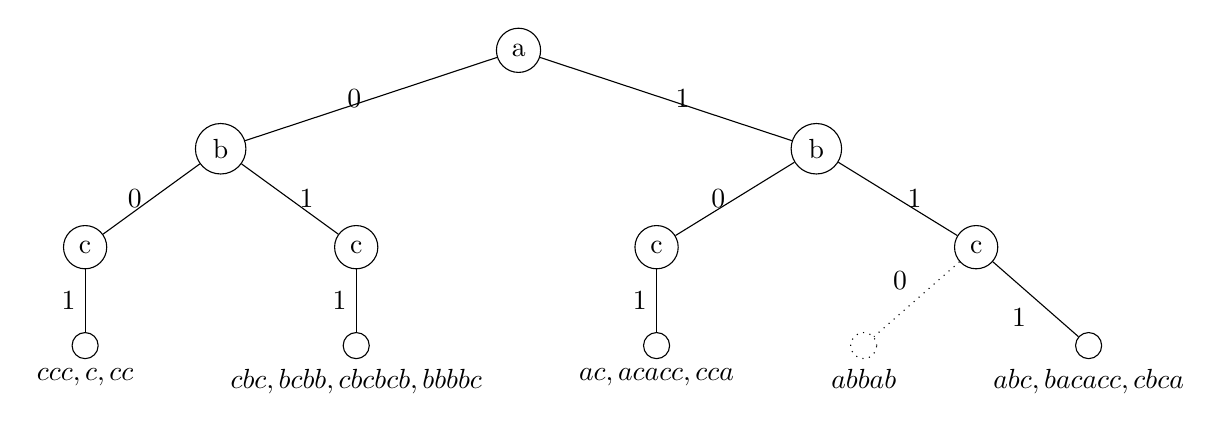
\begin{tikzpicture}[every tree node/.style={draw,circle},
	level distance=1.25cm,sibling distance=1cm,
	edge from parent path={(\tikzparentnode) -- (\tikzchildnode)}]
	\Tree 
	[.a 
		\edge node[midway,left] {$0$};
		[.b
			\edge node[midway,left] {$0$};
			[.c
				\edge node[auto=right] {$1$};
				[.\node [label=below:${ccc,c,cc}$] {}; ]
			]
			\edge node[midway,right] {$1$};
			[.c
				\edge node[auto=right] {$1$};
				[.\node [label=below:${cbc,bcbb,cbcbcb,bbbbc}$] {}; ] 
			]
		]
		\edge node[midway,right] {$1$};
		[.b
			\edge node[midway,left] {$0$};
			[.c
				\edge node[auto=right] {$1$};
				[.\node [label=below:${ac, acacc, cca}$] {}; ]
			]
			\edge node[midway,right] {$1$};
			[.c
				\edge [dotted] node[auto=right] {$0$};
				[.\node [dotted,label=below:${abbab}$] {}; ]
				\edge node[auto=right] {$1$};
				[.\node [label=below:${abc, bacacc, cbca}$] {}; ]
			]
		]	
	]
	\end{tikzpicture}
	

			
\end{center}
\end{figure}

\subsection{Matching the candidates}
The bit vectors of the candidate set are matched by traversing the vectortree, based on the values of the bit vector generated for that candidate. If a path to a leaf node exists, all the target registrations in the leaf node are considered a match, and if no such leaf node can be reached, the candidate is discarded. Tree-traversal is done by exploring all the possible branches in the tree, but a branch is pruned if the difference between the current path and path corresponding to the bit vector (that is, all the paths which labels correspond to the values of the bits in the bit vector) exceeds some predefined threshold.  
\newline

Since the matches are based on the values of the bit vectors, the strings of the matches do not necessarily need to be exactly the same. Therefore, the Levenshtein distance is used to calculate the exact distance. However, since the bit vector groups certain letters into a single group, potential matches that are within the Levenshtein distance could be missed when only taking the leaf node on the direct path into account. 
For example, when matches with an edit distance of 1, the legitimate match between the names \textit{Zegers} and \textit{Segers} will not be in the same leaf node and therefore are not considered to be a match when only taking the matches into account that are in the same leaf node. For example: the bitvector of the names \textit{Zegers} and \textit{Segers} are $\langle 1, 0, 1, 0, 0, 1, 0, 0\rangle$ and $\langle 1, 0, 1, 0, 0, 0, 1, 0\rangle$, respectively. Upto bit 5, these vectors are completely the same, and therefore follow the same path.
\newline

In order to compensate for this, the paths that are accessible within the maximum error are also considered, and the registrations in the corresponding leaf nodes are added to the set of potential matches.

\section{Matching with higher thresholds}
\subsection{Name pair matching}
\label{sec:name_pair_matching}
In the method described above, the edit distance is calculated over the strings of all four names. This could lead to false negatives: the maximum edit distance is exceeded and the match is rejected, but the match should have been accepted. There are many names in the Dutch language that have alternative writing styles. Examples are first names like \textit{Cornelis} / \textit{Kornelis} and \textit{Lourens} / \textit{Laurens} or surnames like \textit{Huizen} / \textit{Huijzen} or \textit{Belsen} / \textit{Belzen}. 
The similarity between these name variants is that the variants share the same semi-phonetic form, although the spelling is different. This adds at least a cost of 1 to the (levenshtein) edit distance, where there is a good reason to ignore these kinds of name variants. 



% Voorbeeld toevoegen
In \cite{bloothooft2014learning} a set of decision rules was proposed to accept matches based on the edit distance per name. Matching was done not only based on edit distance, but also on the additional constraint that matches must share the same prefix. This was done in order to accept matches for name pairs with higher Levenshtein distances. The constraint on the length of the shared prefix is determined by the edit distance between the two matches, as shown in table \ref{tab:Ruleset}. The constraint on the length demands that, for a given length, either the shortest or the longest name in the name pair is of a certain length (depending on the length of the distance), and the constraint on the prefix demands that both names start with the same sequence of characters. There is also an additional rule, demanding that if the the length of the concatenation of both names minus the edit distance is greater than 16 and the names start with the same letter, the match is also accepted.

\begin{table}
	\centering
	\caption[Extra rules for name based matching]{\label{tab:Ruleset} The set of extra rules when matching is done on single names. The rules are more strict when the Levenshtein distance increases. }
	\vspace{0.5cm}
	\begin{tabular}{ccc}
		\toprule
		Levenshtein distance & length & length matching prefix \\
		\midrule
		1 & shortest $>$ 4 & 1 \\
		2 & shortest $>$ 4 & 2 \\
		3 & longest $>$ 5 & 3 \\
		4 & longest $>$ 7 & 4 \\
		5 & longest $>$ 8 & 4 \\
		\midrule
		\multicolumn{2}{c}{total length of pair minus Levenshtein distance $>$ 16} & 1 \\
		\bottomrule
	\end{tabular}
\end{table}

\subsection{Allowing more distance}
Although \cite{bloothooft2014learning} applied these rules to name pairs for which the names have been converted into semi-phonetical form, we can use these rules to see if any matches that were rejected while using the vectortree technique, which matches on the entire string, can be accepted when looking at the distribution of the Levenshtein distance over the four names in the strings. 
We will focus on the matches with Levenshtein distance 4 and 5, where we accept matches with an Levenshtein distance of 4 or 5 if and only if all of the names of these matches are accepted by the rules in table \ref{tab:Ruleset}. These rules will give some certainty about the extent to which the names match and therefore can be used to make a more informed decision about the gravity of the mismatch of the strings. When a name pair passes the tests in table \ref{tab:Ruleset} there is at least some overlap in that name pair, and the names are of sufficient length to make sure that the edit distance is in some proportion to the length of the names.\\

Figure \ref{fig:4.1} shows the distribution of the length of the names in the matches generated by the set of marriage candidates, categorized by the type of name (first name, surname) and the sex of the person, which shows that for most categories, 75\% of the names have a length of 8 or less. This means that, when looking at matches with Levenshtein distance 4 and 5, the constraint on the length of the matching prefix is a sensible constraint in order to make sure that the error is in proportion to the length of the name. In order to check this, we have created two sets of matches for the matches of the birth-certificates: a set where this constraint was dropped and a set where this constraint was applied. By comparing the number of matches that are dropped when the filtering is applied as described in the next section, the effectiveness of the constraint on the prefix can be tested.

\begin{figure}[ht]
	\begin{center}
		\caption[Distribution of the length of names]{The distribution of the length of names on marriage registrations}
		\includegraphics[scale=0.6]{figures/avg_name_length_boxplot.png}
		\label{fig:4.1}
	\end{center}
	
\end{figure}

When looking at the matches with a Levenshtein distance of 4 or 5, the distribution of the error over the names is also a good factor to take into consideration. An error of 4 or 5 in a single name could mean in some cases that more than half of the entire name of the candidate is different from the name of the target. Although the other three names do match completely (since the error is concentrated in a single name), the difference in that single name will render the match dubious. We will not take the type of name the error is in into account, i.e. we will treat an error of 3 in the first name of a male the same as an error of 3 in the last name of a female.  
We limit the matches we take from matches with a distance of 4 and 5 to those where the error is distributed over more than 1 name. For matches with a distance of 5, we will also ignore the matches which we have labeled `2,3` since these matches differ too much in two names. 

\section{Assessment of birth certificate matches}
Using the vectortree technique we will build sets of families. Using the name pairs and table \ref{tab:Ruleset} we can extend these families with all matches that are matched with a Levenshtein distance of 4 or 5, as described above. The next step is to assess the quality of the matching in the first step. 
Although the assessment of the quality of the matches can be done on any arbitrary matching, we will only assess the quality of the matches between the marriage certificates and the birth certificates here. The set of matches of the birth certificates to the marriage certificates of the parents are the most important set of matches to check for consistency, since these matches are directly related to the existence of a person: a person cannot exist if it is not born, although it is good to note that it is possible that birth certificates are missing or that a person migrated to the province of Zeeland before marrying. \\

There are four checks that can be carried out: 
\begin{itemize}
	\item Are the birth events after the marriage of the parents? \\
	Although children can be born before the parents are married, we do not consider these cases. Assuming that all birth events take place after the parents are married simplifies this check significantly. 
	\item Are there at least 10 months between two consecutive birth events within the same family?\\
	It is very unlikely that children will be born within 10 months from each other, since this is biologically almost an impossibility. 
	\item How long is the overall time span of birth events within the same family?\\
	If there is a gap of 20 years between two consecutive certificates, the likelihood that those certificate belong to the same family is smaller than when there is a gap of 5 years. 
	\item How long is the time span between the marriage of the parents and the birth certificate?
	The time span between the marriage and the birth events can not be greater than 25 years. Lowering this range might make this check more discriminative between families of parents and children with the same name, but it might also pose a problem when looking at large families. 
\end{itemize} 

In order to be accepted as a true match, the match must be compliant with all these four criteria.

 


\chapter{Results and discussion}
\section{Initial matching results}
\subsection{Vectortree matching}
When applying the vectortree matching algorithm to the candidate sets and target set, three sets of matchresults are generated. Table \ref{tab:results_from_vectortree} shows some examples of matches made by matching the birth certificates to the target set.

\afterpage{
	\clearpage
	\begin{landscape}
		\begin{table}
			\centering
			\caption[Example of vectortree output]{\label{tab:results_from_vectortree}Some matching results generated by the vectortree algorithm on birth certificates. The names of the groom and bride of the target registration are listed first. The names of the parents mentioned on the registration are listed in the last four columns. The Distance column indicates the edit distance over the two strings of all four names. }
				\resizebox{\columnwidth}{!} {
				\begin{tabular}{cc*4{l}c*4{l}}
					\toprule
					Distance & Target ID & Male first name & Male last name & Female first name & Female last name & Candidate ID & Male first name & Male last name & Female first name & Female last name \\
					\midrule
					2 & 701331 & cornelis & jansen & johanna & ee & 129230 & cornelis & jansen & janna & ee\\
					2 & 701331 & cornelis & jansen & johanna & ee & 161932 & cornelis & jansen & janna & ee\\
					0 & 704975 & francois & orlebeke & anna & ee & 92863 & francois & orlebeke & anna & ee\\
					0 & 704975 & francois & orlebeke & anna & ee & 347965 & francois & orlebeke & anna & ee\\
					0 & 704975 & francois & orlebeke & anna & ee & 373156 & francois & orlebeke & anna & ee\\
					0 & 704975 & francois & orlebeke & anna & ee & 439624 & francois & orlebeke & anna & ee\\
					0 & 704975 & francois & orlebeke & anna & ee & 480756 & francois & orlebeke & anna & ee\\
					0 & 704975 & francois & orlebeke & anna & ee & 524095 & francois & orlebeke & anna & ee\\
					2 & 891300 & jannis & verbrugge & johanna & ee & 71156 & jannis & verbrugge & janna & ee\\
					2 & 891300 & jannis & verbrugge & johanna & ee & 429783 & jannis & verbrugge & janna & ee\\
					1 & 811218 & jannis & reu & maria & eggel & 296559 & jannis & reu & maria & eggee \\
					\bottomrule
				\end{tabular}
			}
		\end{table}
	\end{landscape}
	\clearpage
}


Table \ref{tab:NumberOfMatches} shows the number of generated matches using the vector tree algorithm, per type of match and per maximum edit distance, as well as the number of extra matches that are generated when using a higher threshold compared to the number of matches with a threshold of 3. In total there are 130,277 extra matches with an edit distance of 4, and 317,287 extra matches with an edit distance of 5.\\
As expected, the number of matches increases strongly when increasing the threshold. 
 
 \begin{table}[ht]
 	\centering
 	\caption[Number of matches of vectortree per maximum edit distance]{The number of matches per maximum edit distance.\label{tab:NumberOfMatches}}
 	\begin{tabular}{llccclcccc}
 		\toprule
 		&& \multicolumn{3}{c}{Number of matches} && \multicolumn{4}{c}{Extra number of matches}\\
 		\cmidrule{3-5} \cmidrule{7-10}
 		Certificate type		&& th $\leq$ 3 & th $\leq$ 4 & th $\leq$ 5 && \multicolumn{2}{c}{th $\leq$ 4} & \multicolumn{2}{c}{th $\leq$ 5} \\
 		\cmidrule{1-1}\cmidrule{3-5} \cmidrule{7-10}	
 		marriage v.s. birth 	&& 556,549 & 610,645 & 741,555 && 54,096 & 109.72\% & 185,006 & 133.24\% \\
 		marriage v.s. marriage	&& 247,494 & 276,097 & 348,051 && 28,603 & 111.58\% & 100,557 & 140.63\% \\
 		marriage v.s. death 	&& 394,251 & 441,829 & 556,252 && 47,578 & 112.06\% & 162,001 & 141.09\% \\
 		\bottomrule\\
 		\multicolumn{5}{r}{Total extra matches:} && 130,277 & & 447,564 &\\
 		\bottomrule
 	\end{tabular}
 	
 \end{table}
 
Figure \ref{fig:dist_ed_per_th} shows the distribution of the error over the names. The edit distance per name pair is used as the labels for a match: if there are 4 names where the edit distance between the names on the target registration and the candidate registration is 1, the label `1,1,1,1' was assigned to that match, and if there is a match with an edit distance of 3 in a name and a name with an edit distance of 1, the label `1,3' is assigned to that match. The order in which the errors occur is not taken into account, as we treat an error in a first name the same as an error in a last name.\newline

The figure shows that a lot of matches have been generated where the error is concentrated in a single name. 55.9\% of all matches with a distance of 3 have the label 3, which means that the entire allowed error of 3 is concentrated in a single name. The same pattern can be seen for matches with an error of 4 and 5. 62.1\% of all matches with an error of 4 have a label of 4 and 46.1\% of all matches with an error of 5 have a label of 5.\\ 

In the vectortree matching, we assumed that all matches with an error of 3 can be accepted. Although an edit distance of 3 over the entire string seems as a sensible measure, these figures show that a lot of matches were generated where the error is concentrated in a single name. Since the average length of a name is between 6 and 7 characters, an error of 3 in a single name means that, on average, the names on the target and candidate registration differ in almost half of the number of characters. This suggests that the assumption that matches where the error is concentrated in a single name should be ignored when looking at higher edit distances is valid, while matches where the error is spread over multiple names can be considered as proper matches. 
\newline


Figure \ref{fig:dist_ed_per_name} shows the number of matches where the maximum distance is concentrated in a single name, broken down by the name type, for the set of matches where the candidate set is the set of marriage registrations of the children. This shows that increasing the threshold will primarily generate more matches in the family name, as discussed above and as indicated in chapter 3, since the number of matches where the error is concentrated in a single first name does not increase as much as the number of matches where the error is concentrated in the last name.


\begin{figure}
	\begin{center}
		\caption[Distribution of the maximum error over the names]{The distribution of the maximum allowed edit distance over the names for all the generated matches, grouped by error per name.}
		\centerline{\includegraphics[scale=0.45]{figures/distribution_max_error_over_names_all.png}}
		\label{fig:dist_ed_per_th}
	\end{center}
	
\end{figure}

\begin{figure}
	\begin{center}
		\caption[Count max error per name]{Breakdown of the number of matches where the maximum allowed edit distance is concentrated in a single name for the matches generated on the marriage certificates.}
		\centerline{\includegraphics[scale=0.45]{figures/distribution_max_error_per_name_mar.png}}
		\label{fig:dist_ed_per_name}
	\end{center}
	
\end{figure}

\subsection{Overlinking and underlinking}

\begin{table}[ht]
	\centering
	\caption[Degree of overlinking per maximum edit distance]{The degree of overlinking per maximum edit distance. The overlinking is expressed as the number of parents linked per (unique) candidate certificate. The candidate certificates are the birth, marriage and death certificates of the children. \label{tab:OverlinkingMatches}}
	\vspace{0.25cm}
	\begin{tabular}{llccclccc}
		\toprule
		&& \multicolumn{3}{c}{Number of unique candidates} && \multicolumn{3}{c}{Average match per candidate}\\
		\cmidrule{3-5} \cmidrule{7-9}
		Certificate type		&& th $\leq$ 3 & th $\leq$ 4 & th $\leq$ 5 && th $\leq$ 3 & th $\leq$ 4 & th $\leq$ 5\\
		\cmidrule{1-1}\cmidrule{3-5} \cmidrule{7-9}	
		marriage v.s. birth 	&& 540,401 & 557,647 & 573,730 && 1.03 & 1.10 & 1.29\\
		marriage v.s. marriage	&& 142,414 & 147,218 & 154,033 && 1.74 & 1.88 & 2.26\\
		marriage v.s. death 	&& 390,960 & 401,082 & 422,082 && 1.01 & 1.10 & 1.32\\
	 	\bottomrule
	\end{tabular}
\end{table}
Table \ref{tab:OverlinkingMatches} shows the average number of matches generated per \textit{unique candidate} certificate. This is a measure on the overlinking results of the matching algorithm, as this table shows the (average) number of target certificate that each unique candidate certificate is matched to. For instance: with a threshold of 5, on average, each birth certificate is matched to 1.29 marriage certificate. To make this more concrete: on average, the matching algorthm found 1.29 pair of parents for each birth certificate when matching with a threshold of 5.\\

The average number of matches per candidate certificate for the birth- and death certificates for the matches with a maximum threshold of 3 is close to 1, which indicates that, on average, each candidate certificate is matched to a target certificate. This shows that, overall, the vectortree algorithm is able to match the candidate certificates very precisely to the target certificates for this type of certificates. \\

For marriage certificates, the expected average number of matches per candidate certificate should be around 2, as there are 2 pairs of parents present on each unique candidate certificate. However, the average number of matched target certificate is 1.74. This means that for these certificates there are actually matches missing, and the results from the vectortree algorithm show that there is a situation of underlinking. \\

As can be seen in table \ref{tab:NumberOfMatches} the vectortree algorithm generates 11\% more matches on marriages, when the threshold is increased to 4, but uses only 3.4\% more unique candidates (table \ref{tab:OverlinkingMatches}), and creates 41\% more matches when the threshold is increased to 5 and uses 8\% more unique candidates, compared to a threshold of 3. This shows that increasing the threshold will result in overlinking, as can be expected. This leads to an increase in the average number of match per unique candidate. Because this might not be a situation that is normally acceptable, we will filter out these results in the second and third phase.


\section{Named Pair based matching results}
In total, there are 556,549 matches on birth certificates with a Levenshtein distance of 3 or lower and 54,096 and 130,910 extra matches on Levenshtein distance 4 and 5, respectively. Ignoring the matches with a distance of 4 and 5 as described in section \ref{sec:name_pair_matching}, 20,681 matches remain with a distance of 4, and 34,952 matches remain with an edit distance of 5. \\
There are 247,494 matches for marriage certificates with an error of 3 or lower, and 28,603 and 71,954 matches with an error of 4 and 5, respectively. From the matches with an error of 4, we drop 18,201 matches as the error is concentrated in a single name. This results in 10,402 matches with an error of 4 that we accept. For the matches with error 5 we drop the matches with labels '5` and `2,3'. This means that we drop 52,645 matches and retain the remaining 19,226 matches.\\
Regarding the matches on the death certificates, we have 394,251 matches with a distance of 3 or smaller, 47,578 matches with an error of 4 and 114,423 matches with an error of 5. From the matches with edit distance 4 we drop 29,277 matches and retain 18,301 matches and from the matches with edit distance 5 we drop 83,808 matches and retain 30,615 matches. Table \ref{tab:breakdown_birth_matches} shows the breakdown of the matches that we have retained per label as well as the average number of matched target registrations per unique certificate. \\

The remaining matches with edit distance 4 and 5 are checked for compliance with the rules as described in table \ref{tab:Ruleset}. The acceptance rate for these matches is shown in table \ref{tab:acceptance_rate}. The acceptance rate, which is the ratio of matches that meet all the constraints as described in section \ref{sec:name_pair_matching}, is shown for matches where the additional prefix constraint is not applied (in the `Loose' column) and where the additional constraint is applied (in the `Strict' column). When comparing the acceptance rate for matches with edit distance 4 and 5, the matches with a distance of 5 are clearly less precise. This is expected, as the edit distance itself is a measure of certainty about the correspondence of two strings. Matches where the edit distance is distributed over more than two names seem to be more precise than matches where the error is concentrated on one or two names. This seems to support our assumption that matches with label `4', `1,4', `2,3' and `5' should not be accepted. \newline


\begin{table}
	\begin{center}
	\caption[Breakdown of all matches]{\label{tab:breakdown_birth_matches} A breakdown of matches per type of match. The labels represent the distribution of the error over the names of the matches. The average number of matches shows the degree of overlinking: the average number of target certificate (parent marriage certificates) that are linked to unique candidate certificates.}
	\vspace{0.5cm}
	\hspace*{-1.85cm}
	\resizebox{\columnwidth}{!} {
		\begin{tabular}{*{2}{crrr}crr}
			\toprule
			\multicolumn{11}{c}{Birth certificates}\\
			\toprule
			\multicolumn{3}{c}{Threshold: $\leq$3} & & \multicolumn{3}{c}{Threshold: 4} & & \multicolumn{3}{c}{Threshold: 5}\\
			Label & \# matches & avg. match & & Label & \# matches & avg. match & & Label & \# matches & avg. match \\
			\cmidrule{1-3} \cmidrule{5-7} \cmidrule{9-11} 
			0 		& 374,474 & 1.00 && 1,1,1,1 & 119 		& 1.01	&& 1,1,1,2 	& 224 		& 1.04\\
			1 		& 101,556 &	1.00 && 1,1,2   & 2,554		& 1.01 	&& 1,1,3 	& 3,546 	& 1.04\\
			1,1 	& 19,218  &	1.00 && 1,3 	& 12,821	& 1.05 	&& 1,2,2 	& 2,606  	& 1.03\\
			2 		& 27,656  &	1.00 && 2,2 	& 5,187		& 1.04 	&&  		&   		&\\
			1,1,1 	& 2,148   &	1.00 &&		   	&			&		&&			&			&\\
			1,2 	& 12,777  &	1.01 &&		   	&			&		&&			&			&\\
			3 		& 18,720  &	1.06 &&		   	&			&		&&			&			&\\
			\midrule
			Total: 	& 556,549 &	1.03 && 		& 20,681 	& 1.04	&&			& 6,376		& 1.04\\
			\bottomrule
		\end{tabular}
	}
		\hspace*{-1.85cm}

		\bigskip
	\resizebox{\columnwidth}{!} {
		\begin{tabular}{*{2}{crrr}crr}
			\toprule
			\multicolumn{11}{c}{Marriage certificates}\\
			\toprule
			\multicolumn{3}{c}{Threshold: $\leq$ 3} & & \multicolumn{3}{c}{Threshold: 4} && \multicolumn{3}{c}{Threshold: 5}\\
			Label & \# matches & avg. match & & Label & \# matches & avg. match & & Label & \# matches & avg. match \\
			\cmidrule{1-3} \cmidrule{5-7} \cmidrule{9-11} 
			0 		& 166,849 &	1.47 && 1,1,1,1	& 61	 & 1.00	&& 1,1,1,2 	& 111   	& 1.00\\
			1 		& 44,785  &	1.10 && 1,1,2 	& 1,221  & 1.03	&& 1,1,3 	& 1,907 	& 1.04\\
			1,1 	& 8,234   &	1.03 && 1,3 	& 6,538  & 1.07	&& 1,2,2 	& 1,351 	& 1.03\\
			2 		& 12,027  &	1.03 && 2,2 	& 2,582  & 1.05	&& 			&			&\\
			1,1,1 	& 980     &	1.01 &&			&		 &	&&				&			&\\
			1,2 	& 5,608   &	1.03 &&			&		 &	&&				&			&\\
			3 		& 9,011   &	1.08 &&			&		 &	&&				&			&\\
			\midrule
			Total: 	& 247,494 &	1.74 && 		& 10,402 & 1.06	&&			& 3,369 	& 1.04\\
			\bottomrule
		\end{tabular}
	}
		\hspace*{-1.85cm}

		\bigskip
	\resizebox{\columnwidth}{!} {
		\begin{tabular}{*{2}{crrr}crr}
			\toprule
			\multicolumn{11}{c}{Death certificates}\\
			\toprule
			\multicolumn{3}{c}{Threshold: $\leq$ 3} & & \multicolumn{3}{c}{Threshold: 4} && \multicolumn{3}{c}{Threshold: 5}\\
			Label & \# matches & avg. match & & Label & \# matches & avg. match & & Label & \# matches & avg. match \\
			\cmidrule{1-3} \cmidrule{5-7} \cmidrule{9-11} 
			0 		& 246,288 & 1.00	&& 1,1,1,1 	& 135	 & 1.02	&& 1,1,1,2 	&  202	  & 1.03\\
			1 		& 80,103  &	1.00	&& 1,1,2 	& 2,387  & 1.01	&& 1,1,3 	&  3,106  & 1.03\\
			1,1 	& 16,209  &	1.00	&& 1,3 		& 11,297 & 1.05	&& 1,2,2 	&  2,229  & 1.03\\
			2 		& 22,743  &	1.00	&& 2,2 		& 4,482  & 1.03	&&   		&   	  & \\
			1,1,1 	& 1,910   &	1.00 	&&			&			&&			&&\\
			1,2 	& 11,007  &	1.00 	&&			&			&&			&&\\
			3 		& 15,921  &	1.05	&&			&			&&			&&\\
			\midrule
			Total: 	& 394,181 &	1.01 	&& 			& 18,301 & 1.04	&&			& 5,537   & 1.03\\
			\bottomrule
		\end{tabular}
	}
	\hspace*{-1.85cm}
	\end{center}
\end{table}



\begin{table}
	\begin{center}
		\caption[Acceptance rate]{\label{tab:acceptance_rate} The acceptance rates for edit distance 4 and 5 on the ruleset in table \ref{tab:Ruleset}. The acceptance rate describes the percentage of generated matches per label that comply with these rules. The 'Loose' columns show the acceptance rate of matches when the constraint on matching starting characters is not applied, whereas the 'Strict' columns show the rates where this constraint is applied. }
		\vspace{0.5cm}
		\resizebox{\columnwidth}{!} {
			\begin{tabular}{*{13}{c}}
				\toprule
				\multicolumn{13}{c}{Acceptance rate - Birth $\leftrightarrow$ Marriage  certificates}\\
				\midrule
				\multicolumn{6}{c}{Threshold: 4} && \multicolumn{6}{c}{Threshold: 5}\\
				\cmidrule{1-6} \cmidrule{8-13}
				Label 	& \# matches & \multicolumn{2}{c}{Loose}	& \multicolumn{2}{c}{Strict} && Label 	& \# matches & \multicolumn{2}{c}{Loose}	& \multicolumn{2}{c}{Strict} \\
				\cmidrule{1-2} \cmidrule{3-4} \cmidrule{5-6} \cmidrule{8-13} 
				1,1,1,1 & 119 		& 43.70\% & 52 		& 31.09\% 	& 37 	&& 1,1,1,2 	& 224		& 50.00\% 	& 112	& 33.03\% & 74	\\
				1,1,2 	& 2,554 	& 59.71\% & 1,525 	& 35.83\% 	& 915 	&& 1,1,3 	& 3,546		& 36.91\% 	& 1,309	& 15.48\% &	549 \\
				1,3 	& 12,821 	& 47.35\% & 6,071 	& 18.48\% 	& 2,369	&& 1,2,2 	& 2,606		& 35.03\%	& 913 	& 12.70\% & 331 \\
				2,2 	& 5,187 	& 47.27\% & 2,452 	& 17.27\% 	& 896	&&  		& 	&   	& 	&   &  \\
				\midrule
						& 20,681	& 48.84\% & 10,100 	& 20.39\%	& 4,217	&&			& 6,376	& 36.6\%	& 2,334 & 14.96\% & 954\\
				\bottomrule
			\end{tabular}
		}
		\bigskip
		
		\resizebox{\columnwidth}{!} {
			\begin{tabular}{*{13}{c}}
				\toprule
				\multicolumn{13}{c}{Acceptance rate - Marriage $\leftrightarrow$ Marriage certificates }\\
				\midrule
				\multicolumn{6}{c}{Threshold: 4} && \multicolumn{6}{c}{Threshold: 5}\\
				\cmidrule{1-6} \cmidrule{8-13}
				Label 	& \# matches & \multicolumn{2}{c}{Loose}	& \multicolumn{2}{c}{Strict} && Label 	& \# matches & \multicolumn{2}{c}{Loose}	& \multicolumn{2}{c}{Strict} \\
				\cmidrule{1-2} \cmidrule{3-4} \cmidrule{5-6} \cmidrule{8-13} 
				1,1,1,1 & 61 		& 32.78\% & 20 		& 18.03\% & 11 		&& 1,1,1,2 	& 111		& 44.14\% & 49		& 31.53\% & 35\\
				1,1,2 	& 1,221		& 58.23\% & 711		& 34.46\% & 422		&& 1,1,3 	& 1,907		& 33.67\% & 642		& 15.21\% & 290\\
				1,3 	& 6,538		& 43.27\% & 2,829	& 16.20\% & 1,059	&& 1,2,2 	& 1,351		& 33.46\% & 452		& 12.06\% & 163\\
				2,2 	& 2,582		& 42.72\% & 1,103	& 12.59\% & 325		&&  		& 			&  	 & 	&  & \\
				\midrule
						& 10,402	& 44.83\% & 4,667 	& 17.48\% & 1,817	&&			& 3,369		& 34.22\% & 1,153 	& 14.49\% & 488\\
				\bottomrule
			\end{tabular}
		}

		\bigskip

		\resizebox{\columnwidth}{!} {
			\begin{tabular}{*{13}{c}}
				\toprule
				\multicolumn{13}{c}{Acceptance rate - Death $\leftrightarrow$ Marriage certificates}\\
				\midrule
				\multicolumn{6}{c}{Threshold: 4} && \multicolumn{6}{c}{Threshold: 5}\\
				\cmidrule{1-6} \cmidrule{8-13}
				Label 	& \# matches & \multicolumn{2}{c}{Loose}	& \multicolumn{2}{c}{Strict} && Label 	& \# matches & \multicolumn{2}{c}{Loose}	& \multicolumn{2}{c}{Strict} \\
				\cmidrule{1-2} \cmidrule{3-4} \cmidrule{5-6} \cmidrule{8-13} 
				1,1,1,1	& 135 		& 43.70\% & 59 		& 28.89\%	& 39	&& 1,1,1,2 & 202	& 49.00\% & 99 		& 31.68\% & 64	\\
				1,1,2 	& 2,387		& 60.20\% & 1,437	& 36.57\%	& 873	&& 1,1,3   & 3,106	& 37.54\% & 1,116	& 17.58\% & 546	\\
				1,3 	& 11,297	& 47.48\% & 5,364	& 18.74\%	& 2,117	&& 1,2,2   & 2,229	& 34.99\% & 780		& 14.09\% &	314	\\
				2,2 	& 4,482		& 46.63\% & 2,090	& 16.17\%	& 725	&&   & &   & 	&   & 	\\
				\midrule
						& 18,301	& 48.96\% & 8,961 	& 20.51\%	& 3,754	&&		   & 5,537 & 36.03\% &  1,995	& 16.69\%  & 924\\
				\bottomrule
			\end{tabular}
		}
	\end{center}
\end{table}



\section{Filtering birth certificates}

\begin{figure}
	\begin{center}
		\caption[Consistency check acceptance rate (no prefix constraint)]{\label{fig:consistency_check_loose}Percentage of rejected and accepted matches by the extra checks on consistency. The matches that are checked are the matches that are accepted when name pair based matching is performed without the extra constraint on the matching prefixes. (Loose) }
		\includegraphics[scale=0.45]{figures/rejection_rate_loose.png}
		\caption[Consistency check acceptance rate (with prefix constraint)]{\label{fig:consistency_check_strict} Percentage of rejected and accepted matches by the extra checks on consistency. These matches are the matches that are accepted when name pair based matching is performed with the extra constraint on matching prefixes. (Strict)}
		\includegraphics[scale=0.45]{figures/rejection_rate_strict.png}
		\vspace{0.5cm}
	\end{center}
\end{figure}

The matches on birth certificates that are accepted as described in the previous section are checked for consistency. Figures \ref{fig:consistency_check_strict} and \ref{fig:consistency_check_loose} show the percentages of accepted and rejected matches for the matches with and without the additional matching starting characters constraint, respectively. The name pair matching constraints are only checked for matches with Levenshtein distance 4 and 5.\\
The left plot in both figures shows the number of rejected and accepted matches when the maximum number of years between the first and last birth match is 15 at most, and the right plot shows the same percentages, but when the maximum number of years is 20. In both figures, the number of accepted matches is higher when the maximum allowed years is 20 years. This is expected, as this requirement is less restrictive on the matches. \\

Since matches with a distance of 3 where assumed to be correct matches it is of interest to note that the number of rejected matches increases significantly at edit distance 3. Table \ref{tab:rejection_rate_label} shows that this is mainly contributed by the matches where the distance is concentrated in a single name. Although the majority is accepted by our consistency checks, the rise of the rejection rate suggests that the assumption - that matches with edit distance 3 are safe to accept - must be adjusted and that matches with a distance of 3 in a single name should be investigated further. \\
The effect of additional constraints on matches is clearly visible in the matches with edit distance 4 and 5. With no additional constraint on the prefix, the rejection rate of these matches is around 35\% to 40\% for matches with a maximum of 15 year between the first and last birth certificate. With the additional prefix constraint, the rejection rate drop to between 15\% and 20\%. \\

Table \ref{tab:rejection_rate_label} shows the rejection rate per label. The rejection rate of matches without the additional prefix constraint is lowest when the distance is distributed over all names (or over three in case of a distance of 3), like we expected, and increases as the error is more concentrated in one name, as seen in the previous section. The rejection rate for the matches that comply with the extra prefix constraint seems to be evenly distributed. This is further evidence that the constraint on the prefix of the names can be used in order to distinguish matches when there is a larger distance between the names.


\begin{table}
	\begin{center}
		\caption[Rejection rate per label]{\label{tab:rejection_rate_label}The rejection rate per label shows that the additional prefix constraint filters out a large chunk of the inconsistent matches generated with edit distance 4 and 5 on matches where the maximum difference between the first and last birth certificate in a family is 15 years.}
		\vspace{0.5cm}
	\begin{tabular}{*{4}{l}}
		\toprule
		Distance & Label & Loose & Strict \\
		\toprule
		\multirow{3}{*}{3} & 1,1,1 & 0.057 & 0.057 \\
		& 1,2 & 0.132 & 0.132 \\
		& 3 & 0.433 & 0.433 \\
		\midrule
		\multirow{4}{*}{4} & 1,1,1,1 & 0.115 & 0.162 \\
		& 1,1,2 & 0.087 & 0.079 \\
		& 1,3 & 0.281 & 0.084 \\
		\midrule
		\multirow{4}{*}{5} & 1,1,1,2 & 0.116 & 0.135 \\
		& 1,1,3 & 0.256 & 0.082 \\
		& 1,2,2 & 0.383 & 0.121 \\
		\bottomrule
	\end{tabular}
	\end{center}
\end{table}

\section{Discussion}
Since we do not have a set of matches that we know are correct, it is impossible to compute objective measures of performance for the matching results. However, it is possible to evaluate the performance of the matches on the rule set introduced in the third step of the matching process.\\ 

The distribution of the error over the names for matches with an error of 3 showed that for 55.9\% of these matches the error was concentrated in a single name. This suggest that the assumption that matches with an edit distance of 3 over the entire string of four names are acceptable might be reevaluated, or that the results with an edit distance of 3 should be tested further. The threshold of 3 seems sensible if the error is distributed over all four names. When the error is concentrated in a single name the rejection rate of the consistency check increases, and therefore further analysis is needed for matches with an edit distance of 3.\\

When increasing the threshold for the initial matching algorithm to 4 or 5 in order to be more lenient towards spelling variantions, a lot of extra matches will be generated. As with the matches with an error of 3, care should be taken to accept these extra matches. The vast majority of extra matches will be generated by matches where there is a distance of 3 in a single name. 
When choosing to filter these extra matches on name pairs, the rules as desribed in table \ref{tab:Ruleset} can be used to filter out these unwanted matches. We have tested the ruleset on matches with a maximum edit distance of 4 and 5. The ruleset seems to perform well on both the matches made with distance 4 and 5, as the rejection rate of the matches with these distances that are accepted by this ruleset in the second step of the procedure, and accepted by the consistency checks in the third step of the procedure does not increase significantly when matched with distance 5, compared to matches with distance 4.\\

As can be seen in table \ref{tab:acceptance_rate}, the rules in the second step can filter out a great deal of extra generated matches and are effective in filtering matches that are made with a large distance concentrated in a single name.\\

As mentioned before, there is no way to be certain that the generated matches are actually correct. It is therefore difficult to assess the effectiveness and performance of the approach in this thesis in a coherent, objective way. However, when using edit distance, one can be fairly certain that, with a low edit distance and if consistent with domain knowledge, these matches are indeed proper matches. Whenever the edit distance increases, the matches that are made with a more distributed error are more safe to accept than matches where the error is concentrated in fewer names.

\chapter{Conclusion}
\vspace{-1cm}
This thesis tried to find a method for matching life events taken from historical civil records by looking at the names present on these records. \\

A tree-search algorithm was used to generate matches based on the edit distance of the names on the registrations, where the edit distance varied in order to see if it is possible to account for the high level of spelling variations of these names. The matches where filtered by applying rules to the matches and to filter out those matches where the distance was too much concentrated in a single name. \\
After this filtering, the resulting matches where checked for internal consistency by applying real world logic to the generated matches. \\

When increasing the edit distance, the importance of extra checks on the distribution of the edit distance over the names becomes more important. This can be seen in the number of matches that are dropped in the second step of the method, because of the distribution of the edit distance over the names. \\

Although this thesis provides some judgement on the quality of the matches, it does not evaluate the matches using objective measurements. It is therefore difficult to make a sound conclusion about the effectiveness of the approach. 

\section{Further Research}
For a proper evaluation of the matches generated with a higher edit distance, it might be interesting to conduct clerical review of the generated matches, in order to provide a golden standard for further research. Machine learning algorithmes like active learning might also be used to generate true matches.\\

In order to improve the filtering, the name pair comparison can also be done using name variants, in order make a more informed decision about the nature of the error. Extra rules might be set up for the nature of the error, such as probability rules based on name variants. It also might be interesting to see if name variants evolved throughout time.\\

In the third phase the consistency of the generated sets of families was checked in a fairly basic manner. More thorough checks could be done; for instance by checking the following criteria:
\begin{itemize}
	\item Life course consistency: when the matches on marriage and death registrations are also considered, are there registrations that are inconsistent with the previous matched registrations. For instance: a marriage registration is matched with a event date that is later then a death certificate of that person.
	\item Location / Sex consistency: In the case of two competing registrations, to what extend can the locations on those registration be used to rule out a registration? This could also be checked for the sex of the persons on the registrations.
	\item Name variant consistency: If there are life events missing, are there registrations in the family set where the name of the ego/ega is a name variant of the name for which a certificate is missing? For instance: if the birth and death certificate of \textit{Cornelis} are consistent, but we have a missing marriage certificate and we have a single marriage certificate for a \textit{Cor}, what are the conditions that allow us to accept the marriage certificate of \textit{Cor} to be accepted as the marriage certificate of \textit{Cornelis}?
\end{itemize}

\begin{appendices}
\chapter{Edit distance}
The method that is used to compare a candidate record to a target record is the Levenshtein distance, which is a function to calculate the distance between two strings. The method was introduced by \cite{levenshtein1966binary}. Given two strings \textit{a} and \textit{b}, the distance between \textit{a} and \textit{b} can be defined as the number of operations that need to be executed in order to convert string \textit{a} into string \textit{b} (or \textit{b} into \textit{a}, since the operations are symmetric). \\
The original Levenshtein function assumes three operations: deletion, insertion and substitution of characters in a string, where each operation has a cost of 1. This results in an Levenshtein distance that represents the number of operations. Several variations of the Levenshtein distance exists, where either the cost associated with an operation varies, or the set of operations is altered to allow different operations (such as swapping to characters, also known as transposition) or to disallow certain operations. In our approach, we use the original Levenshtein distance. \\

The Levenshtein distance is calculated in $O(\vert a \vert \times \vert b \vert)$ time, where $\vert \cdot \vert$ denotes the length of a string. This is done by using a dynamic programming algorithm, that uses a matrix with $\vert a \vert + 1$ columns and $\vert b \vert + 1$ rows. Each letter in \textit{a} is associated with a column, and the first column is used for an empty space. An example can be seen in table \ref{tab:LD_example}, where the strings \textit{Peter} and \textit{Pieter} are compared to each other. In order to calculate the Levenshtein distance, the value 0 is assigned to the cell $d[0,0]$ (corresponding to the empty spaces). Then, in a recursive manner, the remaining cells are filled according to the following function:

\begin{equation}
	d[i,j] =
		\begin{cases}
			d[i-1, j-1] & \text{if }a[i] = b[j]\\
			minimum \left\{ 
				\begin{array}{lr}
					d[i-1, j] & \text{(deletion)} \\
					d[i, j-1] & \text{(insertion)}\\
					d[i-1, j-1] + 1 & \text{(substitution)}\\
			\end{array} 
				\right \} & \text{if } a[i] \not = b[j]\\
	\end{cases}
\end{equation} with $0 \leq i \leq \vert a \vert$ and $0 \leq j \leq \vert b \vert$. The resulting value in cell $d[\vert a \vert, \vert b \vert]$ is the final value for the Levenshtein distance between string \textit{a} and string \textit{b}.

\begin{table}
	\begin{center}
	\caption[Example of Levenshtein edit distance]{\label{tab:LD_example}The Levenshtein edit distance for the strings. The bold digits represent the path to the final result. \textit{Peter} and \textit{Pieter}}
	\vspace{0.5cm}
	\begin{tabular}{|c|*{7}{c|}}
		\toprule
		  &   & 0 & 1 & 2 & 3 & 4 & 5 \\ \hline
		  &   & \textvisiblespace & P & e & t & e & r \\ \hline
		0 & \textvisiblespace & \textbf{0} & 1 & 2 & 3 & 4 & 5 \\ \hline
		1 & P & 1 & \textbf{0} & 1 & 2 & 3 & 4\\ \hline
		2 & i & 2 & 1 & \textbf{1} & 2 & 3 & 4\\ \hline
		3 & e & 3 & 2 & \textbf{1} & 2 & 3 & 4\\ \hline
		4 & t & 4 & 3 & 2 & \textbf{1} & 2 & 3\\ \hline
		5 & e & 5 & 4 & 3 & 2 & \textbf{1} & 2\\ \hline
		6 & r & 6 & 5 & 4 & 3 & 2 & \textbf{1}\\ 
		\bottomrule
	\end{tabular}
	\end{center}
\end{table}

\end{appendices}

\listoffigures
\listoftables

\bibliographystyle{apalike}
\bibliography{bibliography_bibtex} 

\end{document}
